\section{Parallelisierung}
\label{sec:parallelpart}
  Im vorherigen Kapitel haben wir die Berechnung der Gravitationskräfte durch Interpolation approximiert. Dadurch konnten wir die Technik der \hquad nutzen, um den Rechenaufwand des Algorithmus zu 
  optimieren.
  Um die absolute Laufzeit aber noch weiter zu reduzieren, sind wir an einer parallel arbeitenden Variante dieses Algorithmus interessiert. In diesem Kapitel wird ein Ansatz dazu vorgestellt.
  
  Ziel ist es, zunächst einen einfachen Algorithmus zu entwerfen. Daher beschränken wir uns auf Parallelisierung nach dem Message-Passing-Modell unter Verwendung von MPI. Wir wollen also 
  $p \in \N$ Prozesse starten können, von denen jeder eine eindeutige $id \in \nullhaken{p-1}$ und seinen privaten Speicherbereich besitzt. Insbesondere ist in diesem Modell Shared-Memory ausgeschlossen. 
  Außerdem sollen die Prozesse miteinander kommunizieren können, um Daten auszutauschen. Die Menge der Prozesse wird im Folgenden mit $\Proc$ bezeichnet.

  Der Code im GitHub-Repository\footnote{https://github.com/AdrianPegler/Gravitation} entspricht der Umsetzung dieses Kapitels inklusive des Vorangegangenen. Da die Methoden durch die Anpassungen
  länger werden, jedoch viel Code durch die vorigen Abschnitte redundant wäre, werden im Folgenden nur noch kurze Codeausschnitte abgebildet. Für allen weiteren Code sei auf das Repository verwiesen.
  
  \subsection{Arbeitsverteilung}
  \label{sec:work}
    Damit wir von parallel arbeitenden Prozessen profitieren können, muss die Arbeit möglichst gleichmäßig auf diese Prozesse verteilt werden. Wir folgen, in modifizierter Variante, dem von 
    \citet{distrh2} vorgestellten Cluster-zentrierten Ansatz. 
    Dieser basiert auf dem Grundgedanken, dass für \vorruck ausschließlich Daten zwischen Vater- und Sohnclustern ausgetauscht werden müssen. Um möglichst viel Kommunikation zu sparen, ist es daher
    besonders effektiv, wenn möglichst viele Söhne durch denselben Prozess verarbeitet werden wie der Vater. Besonders einfach wird das Verteilen der Cluster und das Loadbalancing, wenn wir $p$ als 
    Zweierpotenz $p = 2^q$ wählen. Da dann die Anzahl von Clustern in $T_\Omega^{(q)}$ gerade $p$ entspricht, können wir diese Ebene, zuzüglich der Sohncluster, optimal auf die Prozesse verteilen.
    Wir gehen im Folgenden immer von einer so gewählten Anzahl Prozesse aus.
    
    Um diesen Ansatz auf den Algorithmus zu übertragen, wird in der in \autoref{lst:init} aufgeführten \code{init}-Methode die globale Variable $\tcode{SPLIT_DEPTH} = \log_2(p) = q$ gesetzt. 
    Außerdem bekommt die Datenstruktur \code{Cluster} einen weiteren Member: \code{int active}. In diesem  wird die $id$ des für dieses Cluster zuständigen Prozesses gespeichert.
    
    Zudem gibt es aber noch Cluster auf den Ebenen $T_\Omega^{<q} := T_\Omega^{(0)},\dots,T_\Omega^{(q-1)}$. Um ein Cluster $C \in T_\Omega^{<q}$ zu klassifizieren nutzt jeder Prozess $P \in \Proc$
    mit $id_P$ zwei Konstanten. Gilt für alle Nachfahren $\xoverline{C} \in sons^*(C) \colon$ $\xoverline{C}.\tcode{active} \neq id_P$, so wird der Member $C.\tcode{active}$ auf die \code{int}-Konstante 
    \code{inactive} gesetzt. 
    Gibt es aber Nachfahren $\xoverline{C} \in sons^*(C)$ mit $\xoverline{C}.\tcode{active} = id_P$, so wird der Member $C.\tcode{active}$ stattdessen auf die \code{int}-Konstante \code{semi_active} 
    gesetzt. 
    Inaktive Cluster werden während der \vorruck nicht weiter beachtet. Semi-aktive Cluster berechnen zwar Ersatzmassen, aber nur aus den Ersatzmassen des (semi-)aktiven und nicht des inaktiven 
    Sohnclusters.
    
    \begin{figure}[t]
    \begin{subfigure}{0.9\textwidth}
    \begin{lstlisting}[label=lst:parsetup, caption={Für die Verteilung der Cluster auf die Prozesse angepasste \code{_setup}-Methode.}]
void _setup(Cluster *c, int depth){
  if(depth == SPLIT_DEPTH){
    c->active = ++split_count;
  }

  if(depth < MAX_DEPTH){
    _setup_nonLeafCluster(c, depth);
  }

  if(c->active == semi_active){
    if(c->son[0]->active == inactive && c->son[1]->active == inactive){
      c->active = inactive;
    } else{
      if(c->son[0]->active != world.rank 
	&& c->son[0]->active != semi_active 
	&& c->son[1]->active != world.rank 
	&& c->son[1]->active != semi_active) {
	  c->active = inactive;
      }
    }
  }
}
    \end{lstlisting}
    \end{subfigure}
    \end{figure}
    
    Um diese Einteilung vorzunehmen, wird vorrangig der Code der Methode \code{_setup(...)} (vgl. \autoref{lst:setup}) angepasst. Dieser ist in \autoref{lst:parsetup} aufgeführt.
    
    Zudem bekommt der Konstruktor \code{_new_bound_Cluster}  einen neuen Parameter, um den Member \code{active} des zu konstruierenden Clusters zu initialisieren. Für die
    Konstruktion der Wurzel ist dieser auf \code{semi_active} gesetzt. Danach wird durch die Methode \code{_setup_nonLeafCluster(...)} immer der Wert des Vaters an die Söhne weitergegeben.
    Der zugehörige Code ist in der Datei \code{cluster.c} zu finden und wird im Folgenden kurz erläutert.
    
    Dazu wird zunächst überprüft, ob die \code{SPLIT_DEPTH} erreicht wurde. Ist dies der Fall, wird der Member \code{active} auf 
    die $id$ des zuständigen Prozesses gesetzt. Dies geschieht einfach durch Abzählen. Als nächstes folgt der bereits aus \autoref{lst:setup} bekannte Aufruf, der das Teilen in Sohncluster, das 
    Sortieren der \code{bodies} und die Rekursion beinhaltet. Der letzte Teil wird beim Abbau der Rekursion durchgeführt. Hier wird für eben die Cluster in $T_\Omega^{(<q)}$ überprüft, ob diese 
    auf \code{semi-active} bleiben, oder, falls kein Nachfahre aktiv ist, der Member \code{active} auf \code{inactive} gesetzt wird.
    
    \begin{figure}[b]
      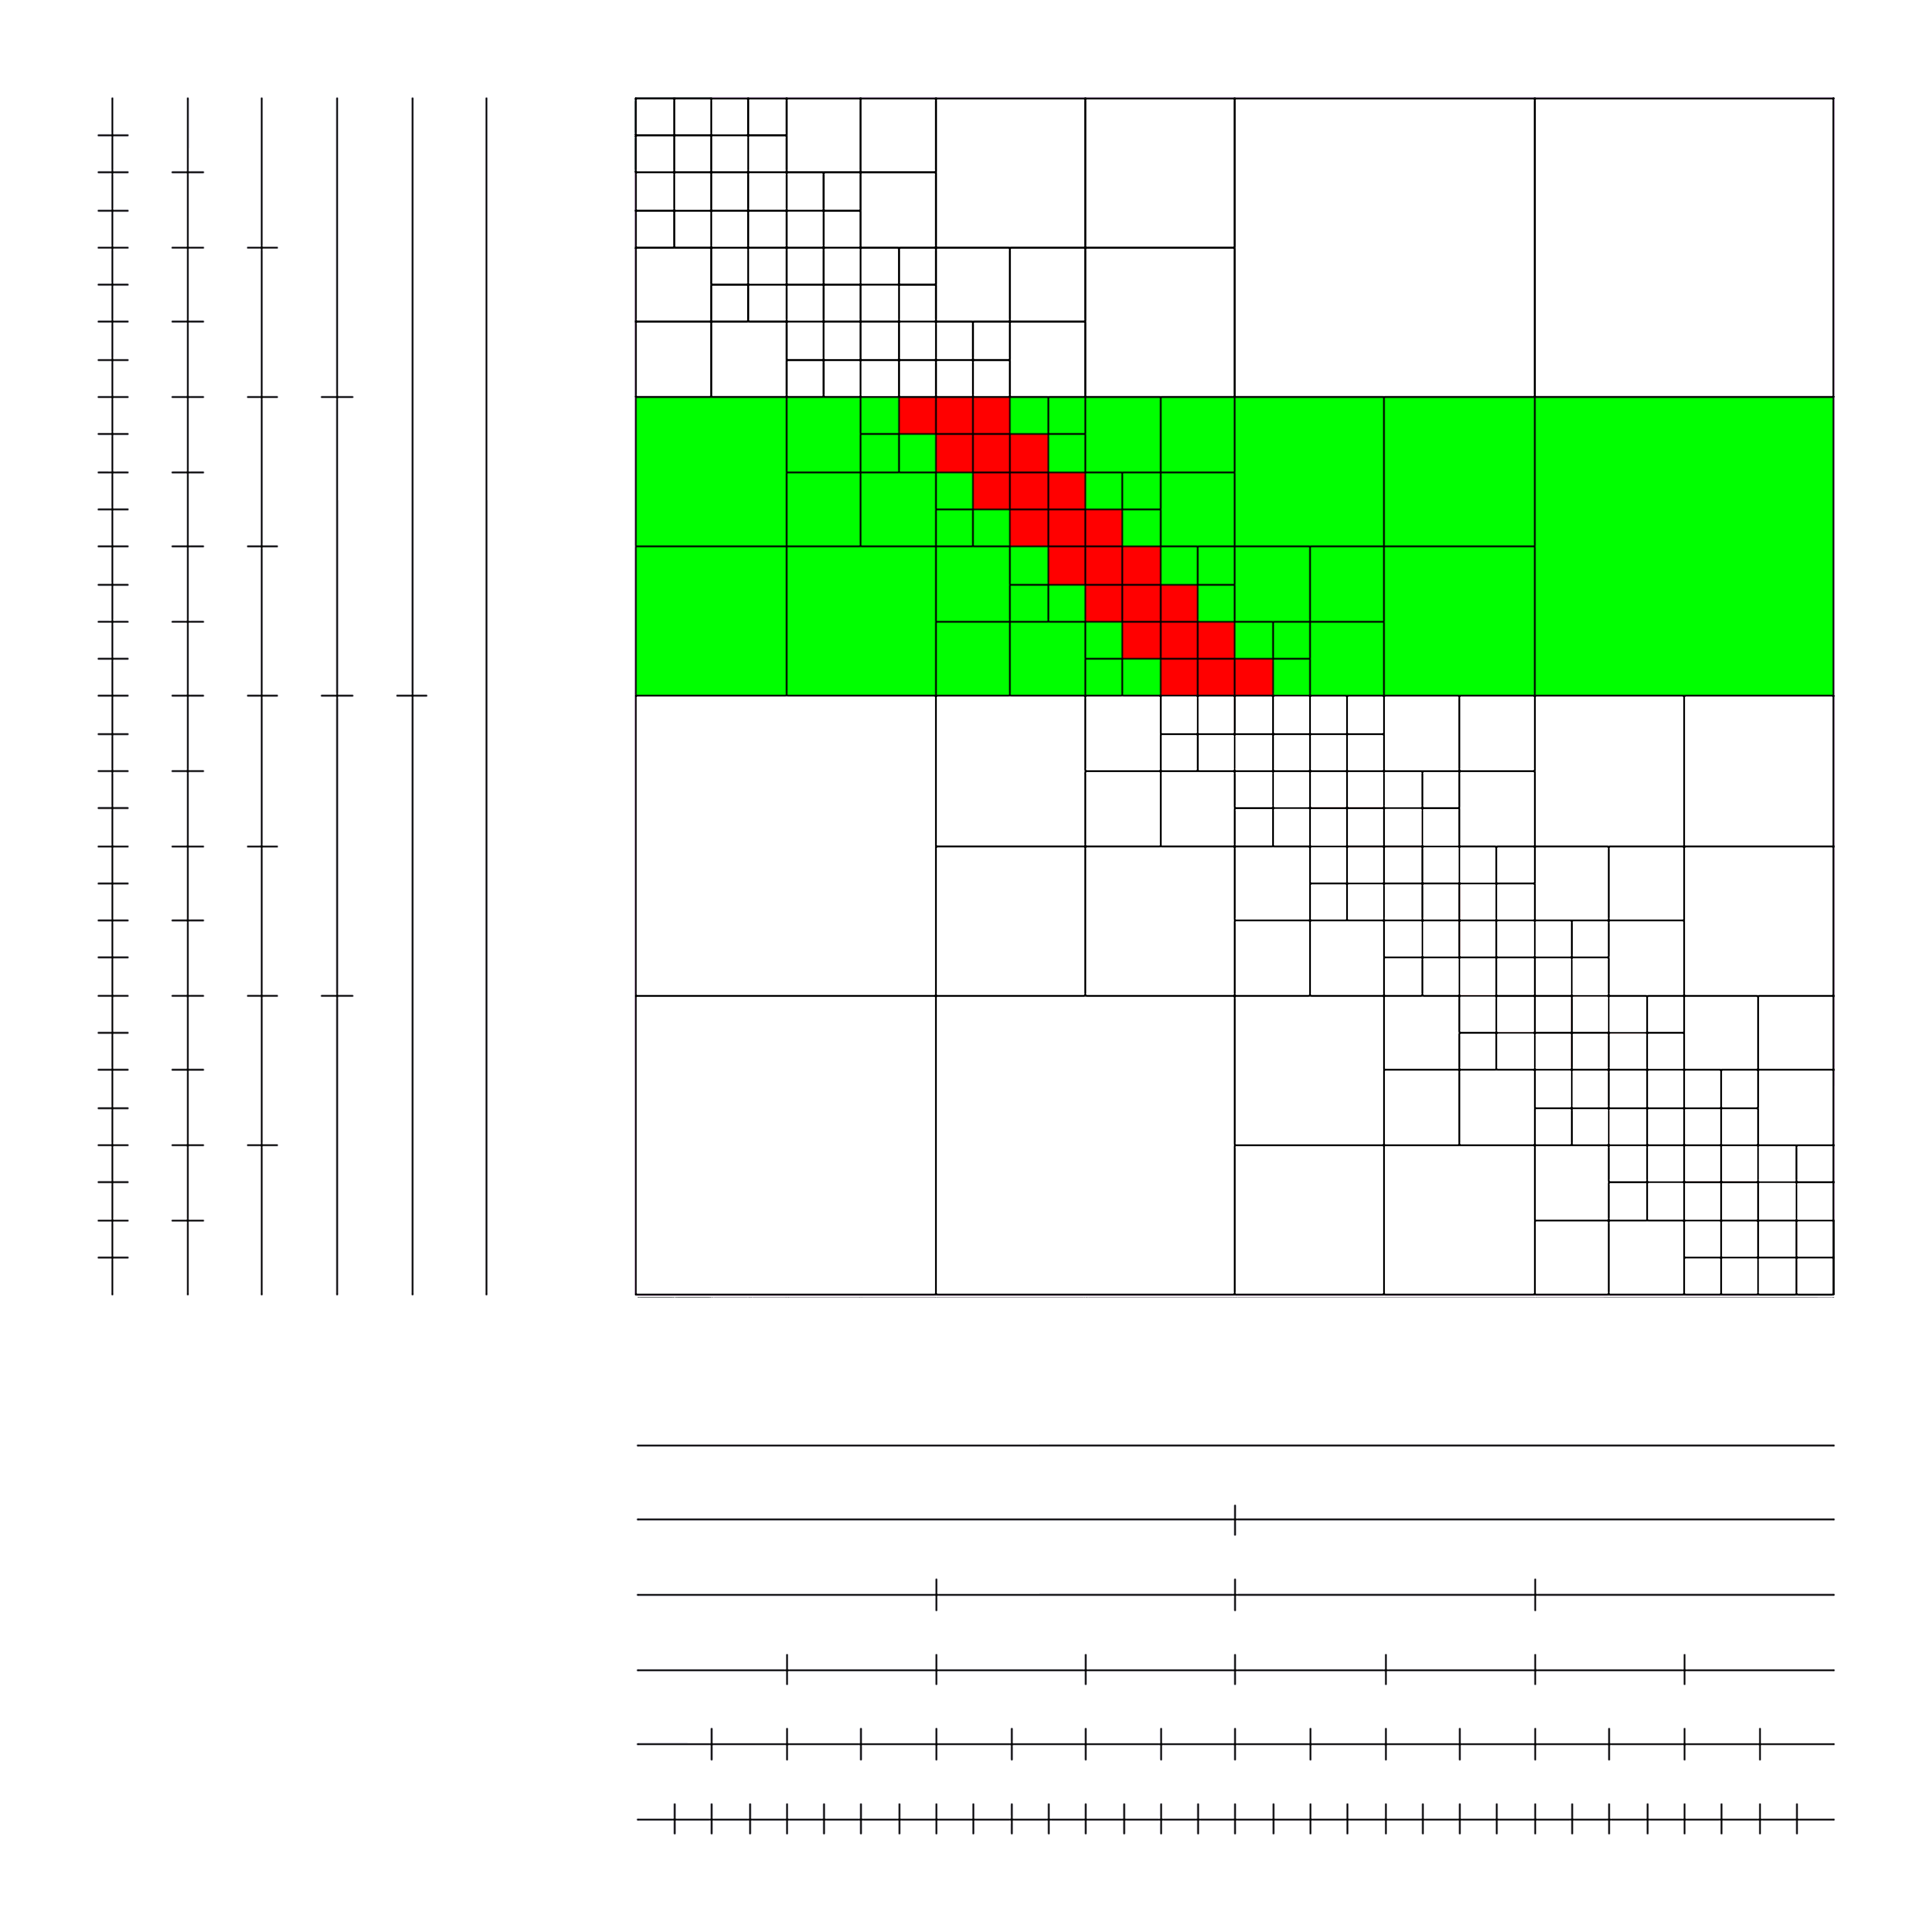
\includegraphics[width=0.8\textwidth]{img/verteilter_blockbaum.png}
      \caption{Für einen Prozess $P$ mit $id_P = 1$ und die Anzahl Prozesse $p = 4$ ist hier die Zuständigkeit des Prozesses $P$ für Blöcke eines Blockbaumes farbig dargestellt.
	       (Quelle: \citet{h2slides})}
      \label{fig:vertblock}
    \end{figure}
    
    Die Idee der semi-aktiven Cluster beruht darauf, die Gestalt der Spalten- bzw. Zeilenmatrizen $V_\tau$ und $W_\sigma$ auszunutzen. Diese werden für Nicht-Blattcluster durch die Transfermatrizen 
    aus den Söhnen konstruiert (vgl. \autoref{sec:approxf}). Während der \vorw werden für ein solches Cluster $C_{semi} \in T_\Omega^{<q}$ die Ersatzmassen nur aus (semi-)aktiven Söhnen
    errechnet. Da diese Cluster für mehrere Prozesse als semi-aktiv gekennzeichnet sind, werden global betrachtet alle Söhne in der \vorw beachtet. Ist eines dieser Cluster Bestandteil
    eines zulässigen Blockes $b_0 = C_{semi} \times C$ oder $b_1 = C \times C_{semi}$, so können die Prozesse ihre Berechnungen untereinander austauschen. Somit werden die Definitionen der Matrizen
    $V_\tau$ und $W_\sigma$ aus \autoref{eq:vtau} beziehungsweise \autoref{eq:wsigma} lediglich auf mehrere Prozesse verteilt und die Summation bei Bedarf aus den Teilergebnissen gebildet.
    
    Unter der Voraussetzung, dass alle notwendigen Informationen für jeden Prozess vorhanden sind, ist die einzige Anpassung der \koppl \kern-0.29em, dass sich die Auswertung auf (semi-)aktive
    Targetcluster beschränkt. Auch die \ruckw wird wiederum lediglich auf (semi-)aktiven Clustern durchgeführt.
    
    Letztlich verteilt sich die Arbeit durch diesen Ansatz sehr natürlich auf die Prozesse. In \autoref{fig:vertblock} ist dies veranschaulicht. Hier ist für einen Prozess $P$ mit $id_P = 1$ 
    und insgesamt $p = 4$ Prozesse dargestellt, welche Zuständigkeit sich für den Prozess $P$ und die Blöcke des Blockbaumes aus der Aufteilung der Targetcluster ergeben. In den Clusterbäumen links 
    und unten sind in hellblau die Clusterbasen, in dunkelblau die Transfermatrizen und in schwarz schraffiert die Transfermatrizen der semi-aktiven Cluster dargestellt.
  
  \subsection{Datenverteilung}
  \label{sec:data}
    
    Eine weitere grundlegende Frage ist, wo welche Daten vorhanden sein sollten. Ein möglicher Ansatz wäre, dass jeder Prozess eine Kopie aller Daten hat. Allerdings würde der Hauptspeicher bei 32 
    Prozessen auf einem Knoten\footnote{Dies entspricht den Spezifikationen der meisten Knoten des RZ-Clusters der Uni Kiel.}  sehr schnell 
    knapp werden. Außerdem sei an dieser Stelle an die weitere Skalierbarkeit des Problems erinnert (vgl. \autoref{sec:parrech}). Daher müssen die Daten über die Prozesse und Knoten verteilt werden. 
    
    Da wir im vorigen Kapitel bereits beschrieben haben, wie die Arbeit effektiv verteilt werden kann, ist es nur naheliegend die Daten auf die gleiche Weise zu verteilen. Jeder Prozess soll also 
    genau die Teile der \code{bodies}-Struktur beinhalten, die zu seinen aktiven Clustern gehören. Dies entspricht den hellblau gekennzeichneten Teilen des Clusterbaumes links in \autoref{fig:vertblock}.
    
    Weder bei reellen Daten noch bei unseren zufällig generierten Testdaten können wir davon ausgehen, dass diese nach Clustern sortiert vorliegen. Da ferner bei reellen Daten davon auszugehen
    ist, dass diese aus Gründen des Speicherbedarfs verteilt eingelesen werden müssen, generiert in unserem Programm ebenfalls jeder Prozess selbst zufällige Testdaten. Es wäre möglich die Daten 
    so verteilt zu belassen, wie sie generiert beziehungsweise eingelesen wurden. Jedoch wäre dann während der \vorruck eine große Menge an Kommunikation notwendig um diese entsprechend der 
    Arbeitsverteilung durchzuführen. Daher ist es sinnvoll diese Daten einmal nach Prozesszugehörigkeit auszutauschen. Dies bedeutet zwar einen erheblichen Kommunikationsaufwand, dafür kann aber im
    Anschluss die \vorruck komplett lokal und ohne weitere Kommunikation durchgeführt werden. Außerdem ist nicht davon auszugehen, dass viele Sonnen ihre bounding box während weniger Simulationsschritte
    verlassen. Daher kann dieser Kommunikationsaufwand als einmalig gewertet werden.
    
    Diese Kommunikation wird während der Konstruktion des Clusterbaumes vorgenommen. Der zugehörige Quellcode ist in \autoref{lst:parconsttree} und \autoref{lst:presort} aufgeführt.
    
    Die Methode \code{preSort(...)} sortiert die \code{bodies}, indem sie den Clusterbaum bis zur Ebene \code{SPLIT_DEPTH} konstruiert. In den Arrays \code{send_count[]} und \code{send_displ[]}
    merkt sich jeder Prozess, wie viele Elemente seiner \code{bodies} und ab welcher Position er an welchen anderen Prozess zu senden hat. Respektive werden in den Arrays \code{recv_count[]} 
    und \code{recv_displ[]} die Anzahlen und Pufferpositionen für die zu empfangenden Daten gespeichert. Diese werden über die Methode \code{MPI_Gather(...)} (vgl. \autoref{fig:kolkom}) zwischen 
    den Prozessen ausgetauscht. So bekommt jeder Prozess von den anderen mitgeteilt, wie viele Elemente er von ihnen gesendet bekommen wird. Die Gesamtgröße der künftigen \code{bodies}-Memberarrays
    wird in \code{new_n} gespeichert.
    
    Der Datenaustausch findet über die Methode \code{MPI_Alltoallv(..)} (vgl. \autoref{fig:kolkom} und \autoref{lst:a2a}) statt. Diese führt mit Hilfe der zuvor konstruierten \code{count}- und 
    \code{displ}-Arrays gerade eine Transformation der ``Prozess-Daten-Matrix'' aus. Dadurch ist es in einem einzigen Kommunikationsschritt möglich, dass jeder Prozess jedem anderen die zugehörigen 
    Daten schickt und respektive von diesem erhält. Danach werden noch einige Variablen aktualisiert und schließlich wird der Clusterbaum wie gehabt vollständig bis zur Ebene \code{MAX_DEPTH} 
    konstruiert. 
    
    In \autoref{sec:konstr} wurde der Programmparameter $\tcode{pot}$ vorgestellt, der die Anzahl an Testsonnen bestimmt. Bei der parallelen Variante generiert jeder Prozess gerade $2^{\tcode{pot}}$
    Sonnen. Die globale Menge $\Omega$ hat also $|\Omega| = 2^q 2^\tcode{pot} = 2^{q+\tcode{pot}}$ Elemente. Daher wird die maximale Baumtiefe $\tcode{MAX_DEPTH} = q + \tcode{pot} - \mathfrak{l}$ 
    gesetzt. Dadurch wird die durchschnittliche Blattgröße von $2^\mathfrak{l}$ Elementen beibehalten. Im Folgenden wird die Zahl $n := |\Omega| = 2^{q+\tcode{pot}}$ für alle \code{bodies} auf allen 
    Prozessen und die Zahl $m := 2^\tcode{pot}$ für die durchschnittliche Anzahl \code{bodies} pro Prozess verwendet.
    
    \begin{figure}[b]
  \begin{subfigure}{0.9\textwidth}
    \begin{lstlisting}[label=lst:parconsttree, caption={Ausschnitt aus der parallelen Konstruktion des Clusterbaumes.}]
Cluster *constructClusterTree(bodies *b){
  [...]
  ////////////////////////////////////////////////////////
  // Sort the bodies; first locally, then globally.
  new_n  = preSort(root, 0);
  new_bs = new_bodies(new_n);
  alltoall_bodies(my_bs, send_count, send_displ, new_bs, recv_count, recv_displ);
  del_bodies(my_bs);
  my_bs = new_bs;
  //reset roots bodies*
  root->bodies = my_bs;
  root->n      = my_bs->n;
  
  //clean up
  
  [...]
}
    \end{lstlisting}
  \end{subfigure}
\end{figure}

\begin{figure}[t]
  \begin{subfigure}{0.9\textwidth}
    \begin{lstlisting}[label=lst:presort, caption={Diese Methode sortiert die lokalen \code{bodies} nach Prozesszugehörigkeit.}]
void preSort(Cluster *c, int depth){
    if(depth == SPLIT_DEPTH){
        c->active = ++split_count;
    
        //get count and start index of data to send to process #split_count
        send_count[split_count] = c->n;
        send_displ[split_count] = split_count == 0 ? 0 : send_displ[split_count - 1] + send_count[split_count - 1];
    
        //if the current knot is the active one: gather counts and displs from the other knots:
        MPI_Gather(&send_count[split_count], 1, MPI_INT, recv_count, 1, MPI_INT, split_count, MPI_COMM_WORLD);
        if(world.rank == c->active){
            new_n = 0;
            for(int i = 0; i < world.size; i++){
                recv_displ[i] = new_n;
                new_n        += recv_count[i];
            }
        }
        
    } 
    [...}] // Sortierung und rekursiver Aufruf
}
    \end{lstlisting}
  \end{subfigure}
\end{figure}

    
  \subsection{Kommunikation}
  \label{sec:komm}
    \begin{figure}[t]
      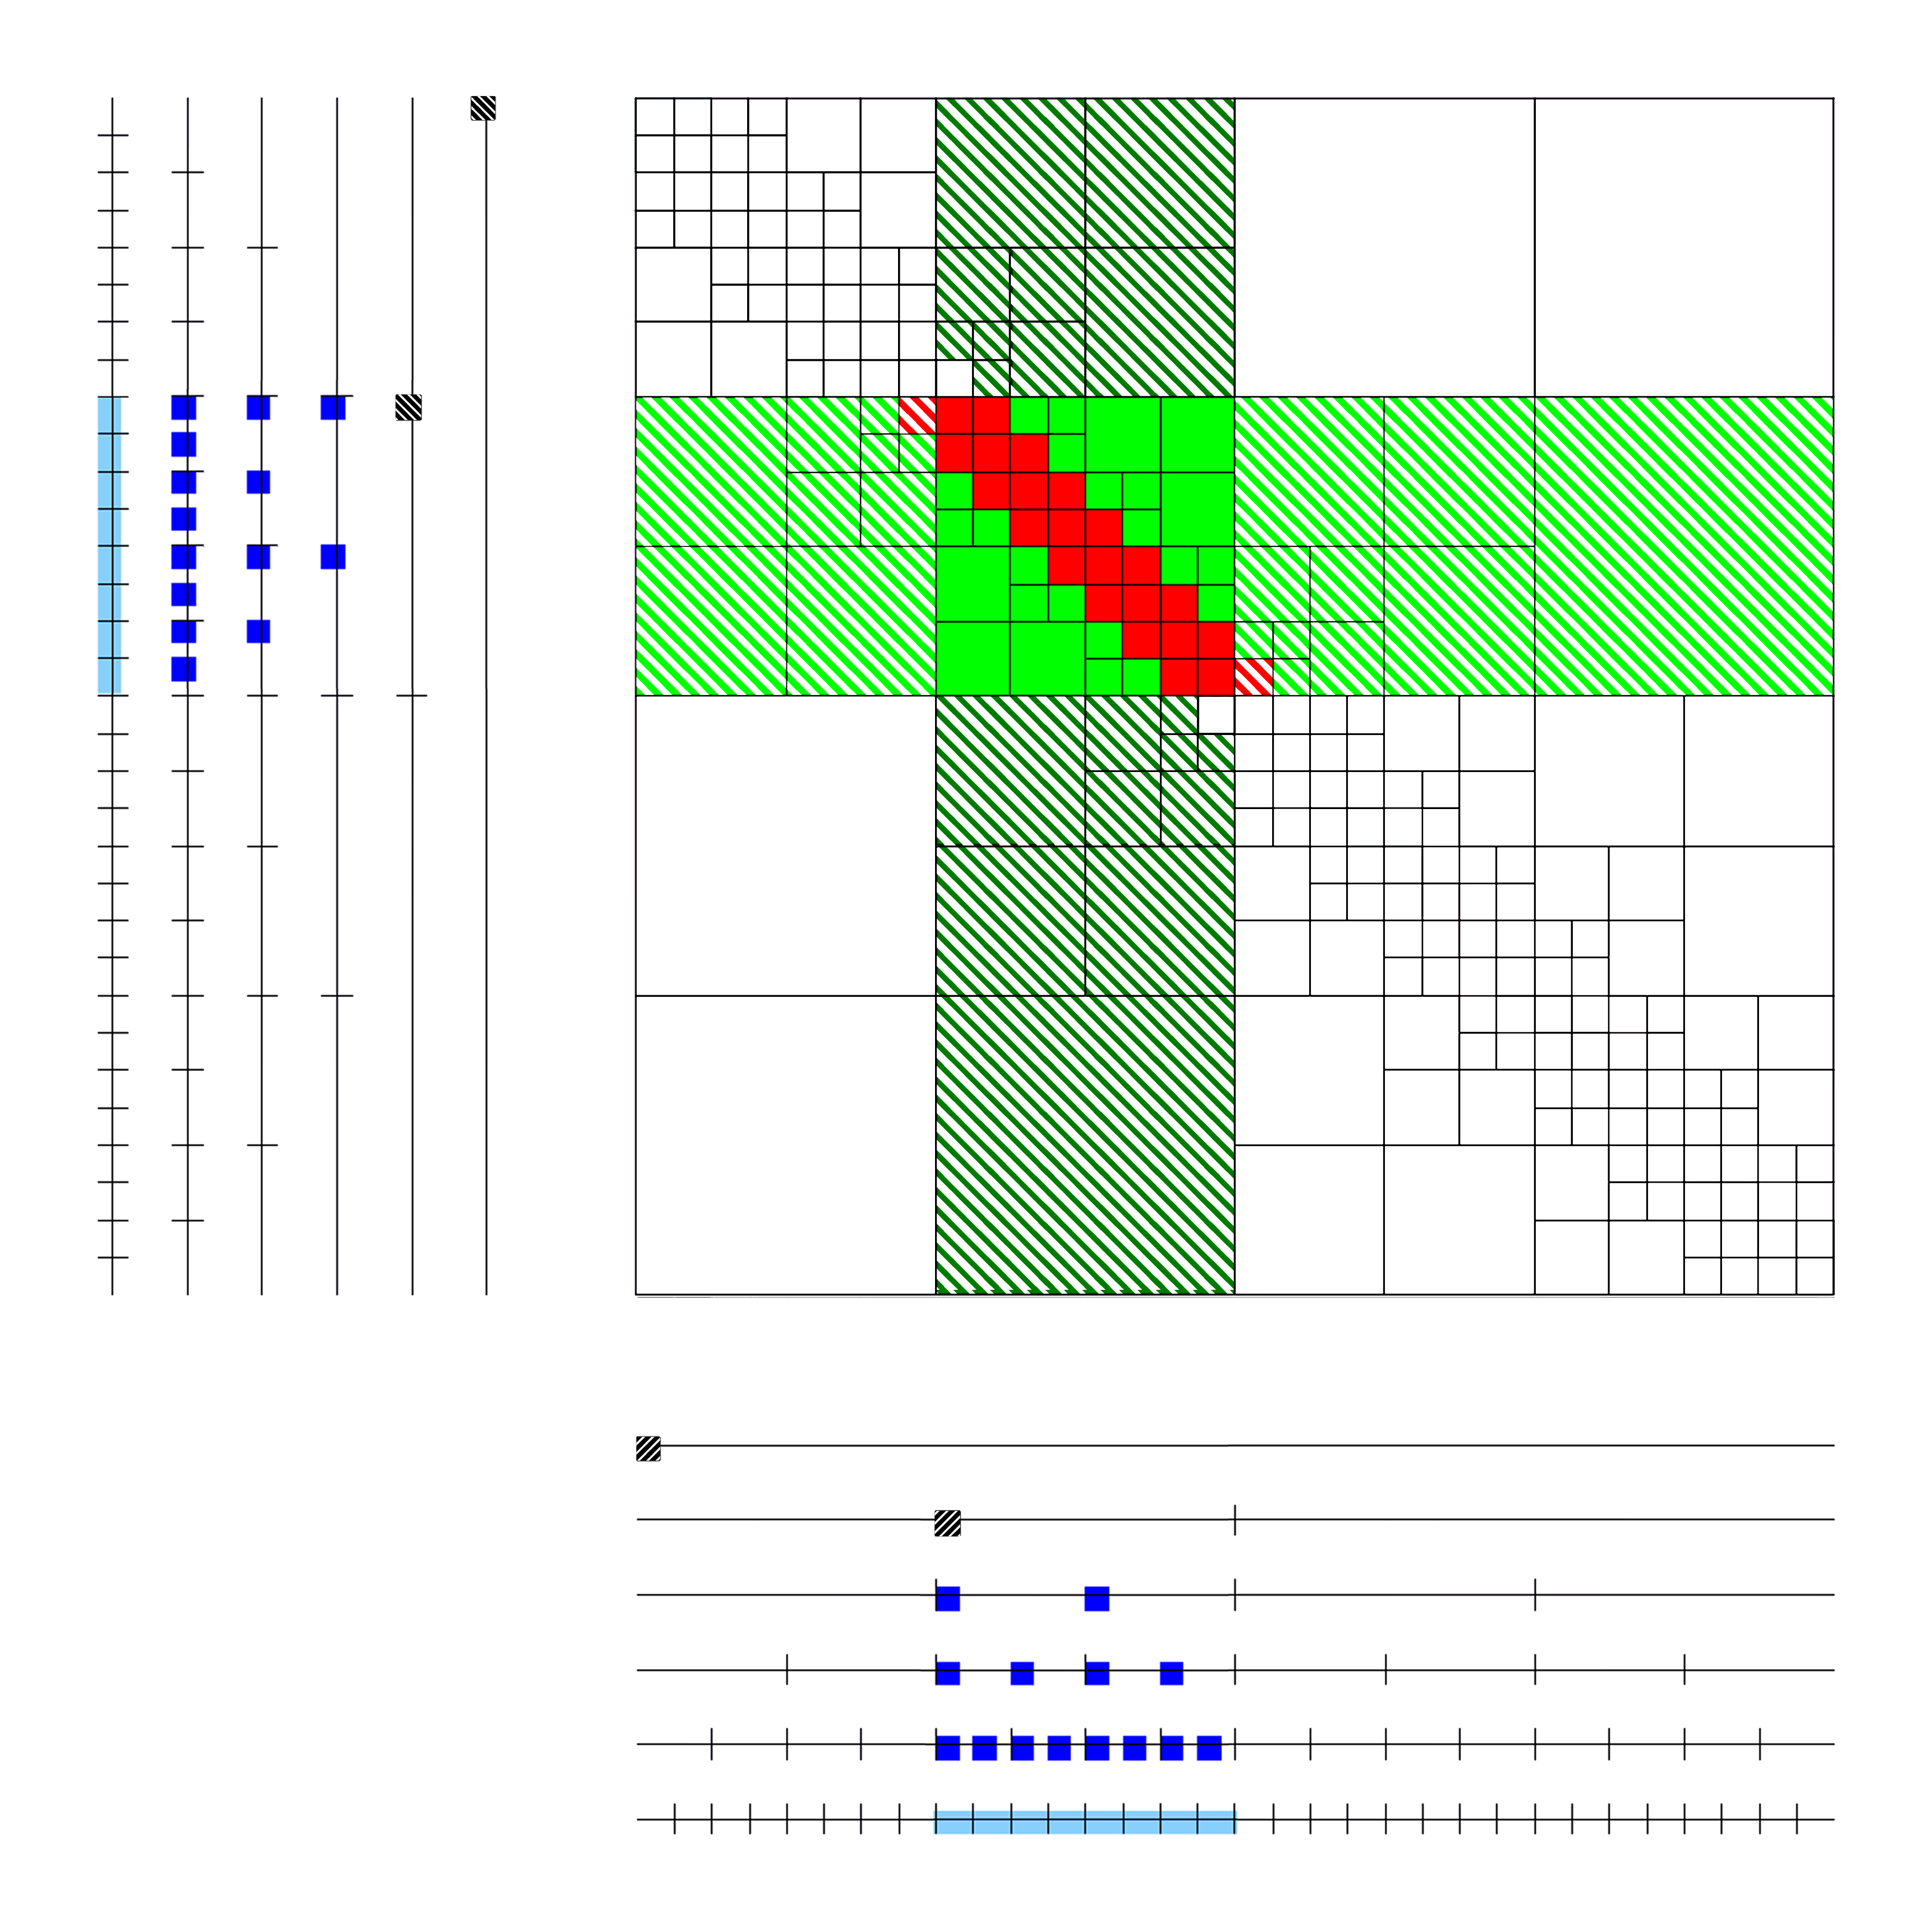
\includegraphics[width=0.85\textwidth]{img/kommimpl.png}
      \caption{Hier sind einige Implikationen der Datenverteilung visualisiert.\\
	       Die schraffierten Blöcke benötigen Datenaustausch mit Prozess $P$\\
% 	       Dunkelgrün schraffiert: Blöcke die Daten von aus der \vorw von $P$ benötigen.\\
% 	       Hellgrün schraffiert: Daten, die $P$ für die \koppl und \ruckw benötigt.\\
% 	       Nicht schraffiert: Blöcke für die alle Daten vorliegen.\\
	       (Quelle: \citet{h2slides})}
      \label{fig:kommimpl}
    \end{figure}

    Als Resultat der Aufteilung der Daten müssen wir uns nun Gedanken machen, welche Daten für die Auswertungen der Matrizen zusätzlich zu den lokal vorhandenen gebraucht und damit kommuniziert werden 
    müssen.
    
    In \autoref{fig:kommimpl} sind diese Zusammenhänge in Bezug auf einen Prozess $P \in \Proc$ visualisiert. Dabei gilt wieder $id_P=1$ und $p=4$. Die dunkel schraffierten Blöcke sind diejenigen, 
    für deren Auswertung Daten von $P$ benötigt werden --
    entweder Berechnungen aus der \vorw für zulässige oder die Daten von Sonnen für unzulässige Blöcke. Der Prozess $P$ muss die Daten aus den zugehörigen Clustern also an die anderen Prozesse 
    übermitteln. Umgekehrt benötigt $P$ die Daten zu den hell schraffierten Blöcken für seine \koppl und \ruckw \kern-0.29em. Lediglich die nicht schraffierten Blöcke benötigen keine Kommunikation, 
    da alle Daten lokal verfügbar sind. Der Datenaustausch kann wie zuvor wieder durch eine Transformation der ``Prozess-Daten-Matrix'' und damit über \code{MPI_Alltoallv(...)} in einem 
    Kommunikationsschritt bewerkstelligt werden. 
    
    Diesmal liegen die Daten allerdings nicht sequentiell hintereinander, sondern sind über den Clusterbaum und die \code{bodies}-Arrays verteilt. Hinzu kommt, dass für zulässige und unzulässige
    Blöcke unterschiedliche Daten ausgetauscht werden müssen. Für zulässige Blöcke brauchen lediglich die errechneten Ersatzmassen ausgetauscht werden, da die Interpolationspunkte bereits von jedem 
    Prozess berechnet wurden. Dies ist also nur ein \code{double}-Array mit verhältnismäßig wenigen Daten.
    Für unzulässige Blöcke hingegen müssen alle zugehörigen Daten aus den Memberarrays \code{x}, \code{y}, \code{z} und \code{m} sowie die Anzahl der zum Cluster gehörenden
    Sonnen übertragen werden.
    
    Auf Grund der Fragmentierung der Daten müssen diesmal für die Kommunikation manuell Sende- und Empfangspuffer angelegt werden. Der zugehörige Code ist in der Datei \code{eval.c} zu finden und wird
    im Folgenden erläutert.
    
    Die Methode \code{void _prep_comm(Cluster *ct, Cluster *cs)} durchläuft ebenso wie die in \autoref{lst:eval} dargestellte Methode \code{_eval(...)} den impliziten Blockbaum und sucht nach 
    zulässigen und unzulässigen Blöcken mit (semi-)aktivem Targetcluster. Pointer zu diesen Source- und Targetclustern werden in Arrays von Vektoren\footnote{Die Implementierung der \code{vector}-Struktur
    sowie zugehörige Methoden wurden von https://\-gist.\-github.com/\-EmilHernvall/953968 übernommen und leicht modifiziert und erweitert.} gespeichert.\footnote{Mit einem Vektor ist in diesem Fall 
    eine Struktur gemeint, die ein Array mit flexibler Länge darstellt.} Dabei wird darauf geachtet, dass die Daten aus (semi-)aktiven Clustern, für die mehrere Prozesse zuständig sind, für alle 
    beteiligten Prozesse vermerkt werden.
    
    Im Anschluss nutzt die Methode \code{void _prep_buffers()} diese gesammelten Daten, um die Sende- und Empfangspuffer zu allozieren und mit den zu sendenden Daten zu füllen. Sind diese Puffer bereit,
    kann die Kommunikation durchgeführt werden. Dazu wird die Methode \code{void _communicate()} aufgerufen. Dies führt mit den entsprechenden Puffern und den gesammelten Anzahl- und Positionsdaten
    insgesamt sechs Aufrufe von \code{MPI_\-Alltoallv(...)} durch: Eine für die Ersatzmassen der Cluster, und fünf für die benötigten \code{bodies}-Daten, da die einzelnen Koordinatenrichtungen, die 
    Anzahlen pro Cluster und die Massen in einzelnen Arrays vorliegen.
    
    Nachdem die Kommunikation vollendet wurde, müssen die Daten noch an die richtigen Stellen vermittelt werden. Die Methode \code{void _finalize_comm()} kopiert die empfangenen Ersatzmassen in die 
    Cluster, in denen diese benötigt werden. Dabei werden die Ersatzmassen von Clustern, die sich aus den Ersatzmassen mehrerer Prozesse zusammensetzen, summiert (vgl. \autoref{eq:vtau} bzw. 
    \autoref{eq:wsigma}). Dies hat den Vorteil, dass wir so später nicht zu unterscheiden brauchen, wo welche Ersatzmassen zu finden sind.
    Die empfangenen \code{bodies}-Daten werden nicht kopiert, um Speicherplatz zu sparen. Die zugehörigen Cluster müssen aber angepasst werden. Der Startindex und die 
    Anzahl wird entsprechend der Empfangspuffer gesetzt. Später können so die Daten direkt aus diesen Puffern abgerufen werden. 
    
    
    Nun kann die \koppl wie gehabt durch Aufrufen der Methode \code{_eval(...)} durchgeführt werden. Die einzigen Anpassungen sind das Auslassen von Blöcken mit inaktivem Targetcluster und die 
    Unterscheidung, ob die \code{bodies}-Daten in der lokalen \code{bodies} Struct oder in den Empfangspuffern zu finden sind.
    
    Abschließend werden die Daten in inaktiven Clustern durch die Methode \code{void _clear_inactive_clusters()} wieder auf $0$ gesetzt, da diese beim nächsten Simulationsschritt nicht überschrieben
    werden würden. (Semi-)aktive Cluster werden während der \vorw neu berechnet und Cluster, für die genau ein anderer Prozess zuständig ist, werden nach der Kommunikation mit den neuen Daten 
    überschrieben. Diese brauchen also nicht eigens geleert werden, um sicherzustellen, dass keine alten Daten verbleiben und zu fehlerhaften Berechnungen führen.
    
    Durch diese Schritte haben wir unseren Algorithmus nun so angepasst, dass Teilprozesse weitestgehend unabhängig voneinander parallel an der Berechnung der Gravitationskräfte arbeiten können.
    Das nächste Kapitel wird noch zeigen, dass diese Arbeitsteilung nahezu optimal ist.